%
\section{Application: Adaptive Viral Marketing} \label{sec:viral-marketing}

For our next application, consider the following scenario.  
Suppose we would like to generate demand for a genuinely novel 
product.  Potential customers do not realize how valuable the new
product will be to them, and conventional advertisements are
failing to convince them to try it.
In this case, we may try to spur demand by offering a special
promotional deal to a 
select few people, and 
hope that demand builds virally, propagating through the social
network as people recommend the product to their friends and
associates.
Supposing we know something about the structure of the
social networks people inhabit, and how ideas, innovation, and new
product adoption diffuse through them, this begs the
question: to which initial set of people should we offer the
promotional deal, in order to spur maximum demand for our product?

\looseness -1 This, broadly, is the viral marketing problem.  
The same problem arises in the context of spreading technological, 
cultural, and intellectual innovations, broadly construed.  In the
interest of unified terminology we 
follow \citet{kempe03} and 
talk of spreading \emph{influence} through the social network, where
we say people are \emph{active} if they have adopted the idea or
innovation in question, and \emph{inactive} otherwise, and that $a$ \emph{influences} $b$ if $a$
convinces $b$ to adopt the idea or innovation in question.

There are many ways to model the diffusion dynamics governing the
spread of influence in a social network.  We consider a basic and
well-studied model, the \emph{independent
  cascade model}, described in detail below. 
For this model~\citet{kempe03}~obtain a very interesting result;
they show that the eventual spread of the influence ${f}$ (i.e., the
ultimate number of customers that demand the product) is a monotone
submodular function of the seed set $S$ of people initially selected.  This, in
conjunction with the results of~\citet{nemhauser78} implies that the
 greedy algorithm 
obtains at least $\paren{1 - \frac1e}$ of the value of the best
feasible seed set of size at most $k$, i.e., $\argmax_{S: |S| \le k} {f}(S)$,
where we interpret $k$ as the budget for the promotional campaign.
Though~\citeauthor{kempe03} consider only the maximum coverage version of
the viral marketing problem, their result  
in conjunction with that of~\citet{wolsey82} also implies that
the greedy algorithm will obtain a quota $Q$ of value at a cost of 
at most $\ln(Q)+1$ times the cost of the optimal set 
$\argmin_{S} \set{c(S) : f(S) \ge Q}$ if $f$ takes on only integral
values. 

 \begin{figure} 
 \centering 
 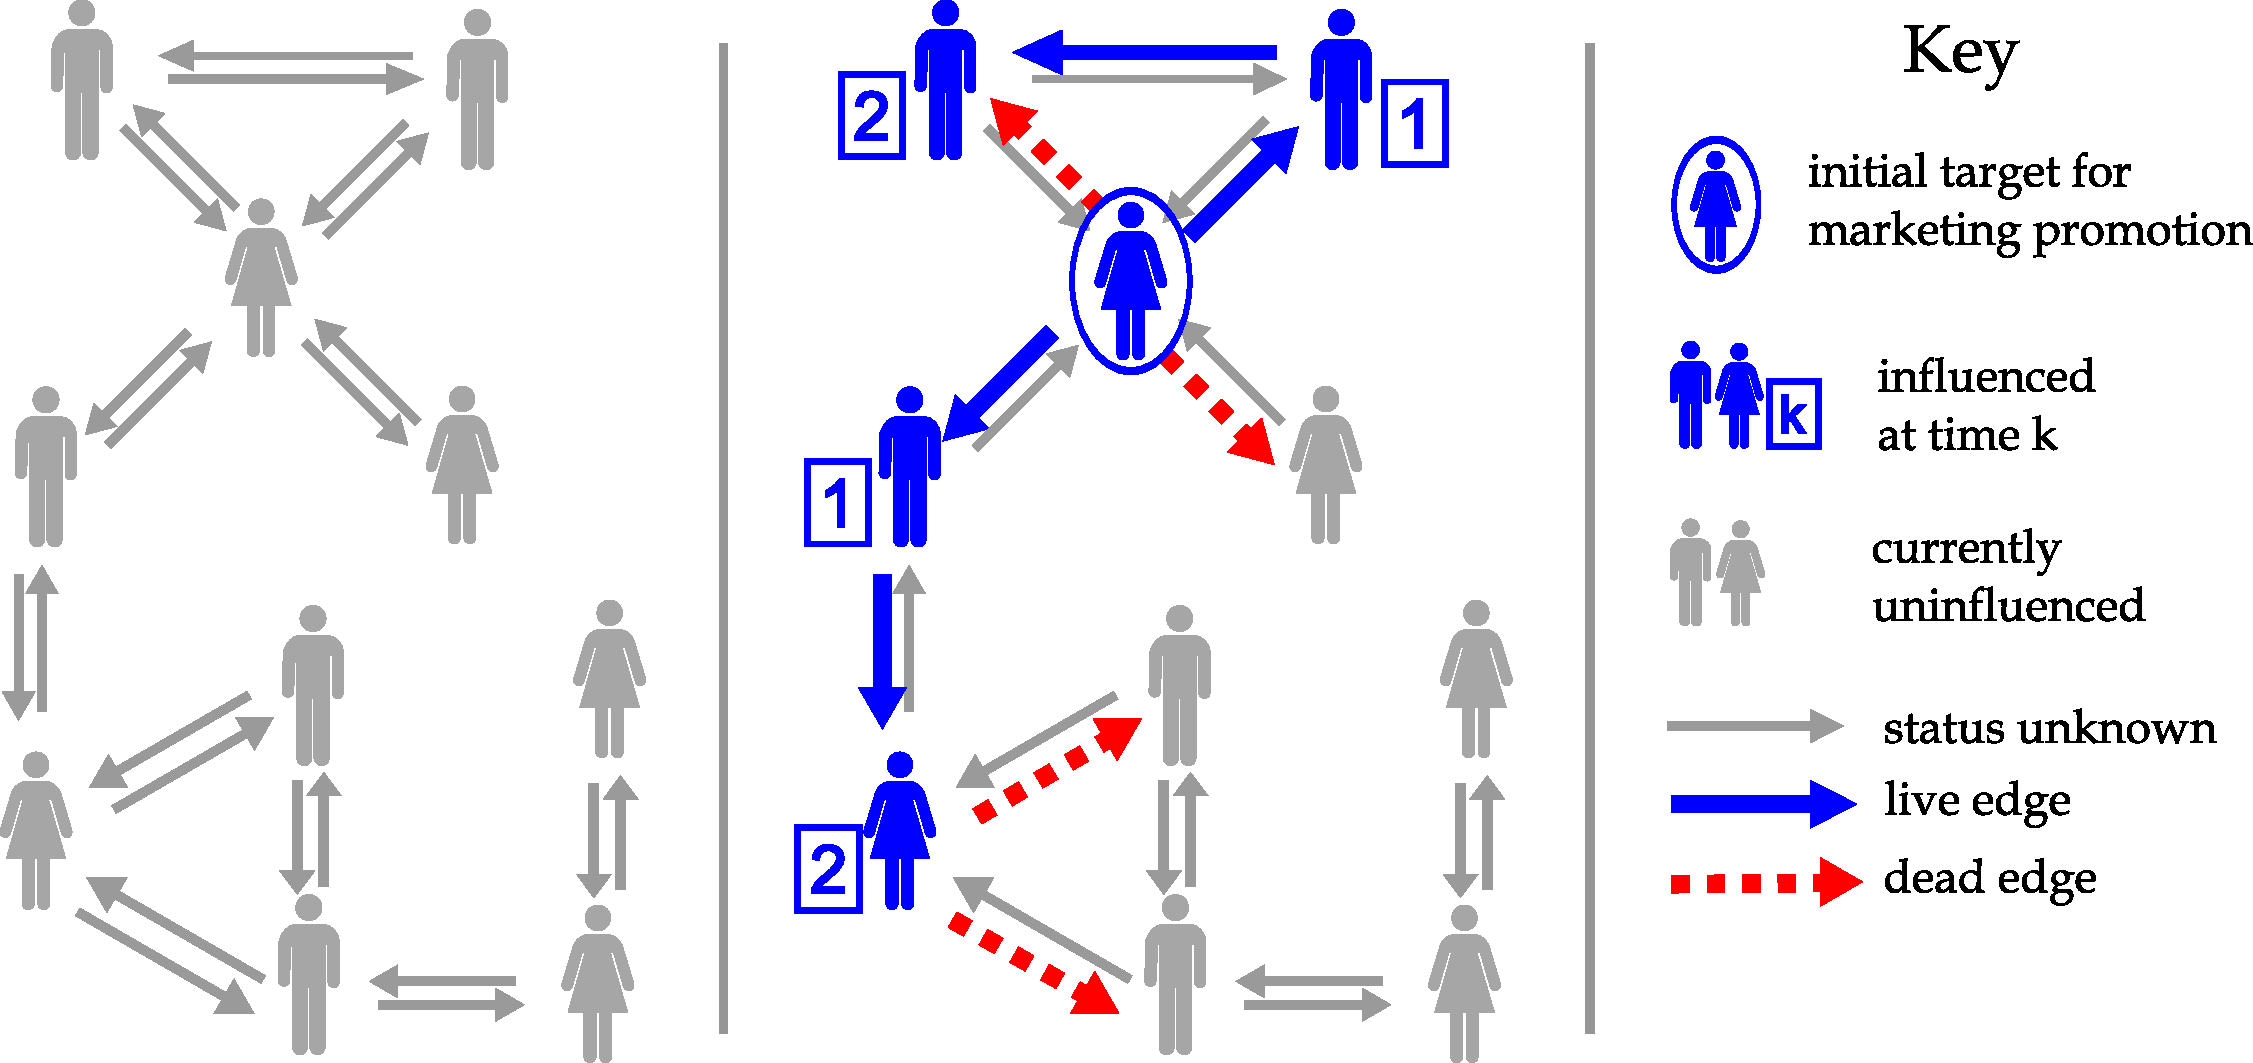
\includegraphics[width=0.8\textwidth]{figs/viralMarketing}
 \caption{Illustration of the Adaptive Viral Marketing problem. Left:
   the underlying social network. 
   Middle: the people influenced and
   the observations obtained after one person is selected.}
 \label{fig:viralmarketing}
 \end{figure}


\subsection{Adaptive Viral Marketing} The viral marketing problem has a very natural adaptive analog. Instead of selecting a fixed set of people in advance, we may select a person to offer the promotion to, 
make some observations about the resulting spread of demand for our product, and repeat. See \figref{fig:viralmarketing} for an illustration.
In \secref{ssec:viral-max-cover}, 
we use the idea of \term submodularity to 
obtain results analogous to
those of \citet{kempe03} in the adaptive setting. 
Specifically, we show that the greedy policy obtains at least $\paren{1 - \frac1e}$ of the value of
the best \emph{policy}.  Moreover, we extend this result by 
achieving that guarantee not only
for the case where our reward is simply the number of influenced
people, but also for any (nonnegative) monotone submodular function of the 
\emph{set} of people influenced.  In \secref{ssec:viral-min-cost-cover}
we consider the minimum cost
cover objective, and show that the greedy policy obtains a logarithmic
approximation for it. To our knowledge, no approximation results for this adaptive variant of the viral marketing problem have been known.




\subsubsection{Independent Cascade Model}
In this model, the social network is a directed graph $G = (V, A)$
where each vertex in $V$ is a person, and each edge $(u, v)\in A$ has an
associated binary random variable $X_{uv}$ indicating if $u$ will
influence $v$.  That is, 
$X_{uv} = 1$ if $u$ will influence
$v$ once it has been influenced, and $X_{uv} = 0$ otherwise.
The random variables $X_{uv}$ are independent, and have known means 
$p_{uv} := \expct{X_{uv}}$.
We will call an edge $(u,v)$ with $X_{uv} = 1$ a \emph{live edge} and
an edge with $X_{uv} = 0$ a \emph{dead edge}. 
When a node $u$ is activated, the edges $X_{uv}$ to each neighbor $v$
of $u$ are sampled, and $v$ is activated if $(u,v)$ is live.
%
Influence can then spread from $u$'s neighbors to their neighbors, and so on,
according to the same process.  Once active, nodes remain active
throughout the process, however~\citet{kempe03} show that this
assumption is without loss of generality, and can be removed.

\subsubsection{The Feedback Model}
In the Adaptive Viral Marketing problem under the 
independent cascades model, the items correspond to people we can 
activate by offering them the promotional deal.  How we define the
states $\rlz(u)$ depends on what information we obtain as a result
of activating $u$.  Given the nature of the diffusion process,
activating $u$ can have wide-ranging effects, so the state 
$\rlz(u)$ has more to do with the state of the social network on the
whole than with $u$ in particular.  
%
%
%
Specifically, we model 
$\rlz(u)$ as a function $\rlz_u:A \to \set{0,1,?}$, where 
$\rlz_u((u, v)) = 0$ means that activating $u$ has revealed that $(u,v)$ is dead, 
$\rlz_u((u, v)) = 1$ means that activating $u$ has revealed that $(u,v)$ is live, and 
$\rlz_u((u, v)) =\ ?$ means that activating $u$ has not revealed the
status of $(u,v)$ (i.e., the value of $X_{uv}$).  We require each
realization to be \emph{consistent} and \emph{complete}.
Consistency means that no edge should be declared both live and dead
by any two states.  That is, for all 
$u, v \in V$ and $a \in A$, $(\rlz_u(a),\rlz_v(a)) \notin \set{(0,1), (1,0)}$.
Completeness means that the status of each edge is revealed by some
activation.  That is, for all 
$a \in A$ there exists $u \in V$ such that $\rlz_u(a) \in \set{0,1}$.
A consistent and complete realization thus encodes $X_{uv}$ for each
edge $(u,v)$.  Let $\alive{\rlz}$ denote the live edges as encoded by
$\rlz$.  
There are several candidates for which edge sets we
are allowed to observe when activating a node $u$.
Here we consider what we call the \emph{Full-Adoption Feedback Model}: 
After activating $u$ we get to
  see the status (live or dead) of all edges exiting $v$, for all  
  nodes $v$ reachable from $u$ via live edges (i.e., reachable from
  $u$ in $(V, \alive{\rlz})$, where $\rlz$ is the true realization. 
We illustrate the full-adoption feedback model in~\figref{fig:viralmarketing}.

\subsubsection{The Objective Function}
In the simplest case, the reward for influencing a set $U \subseteq V$
of nodes is $\hat{f}(U) := |U|$.  \citet{kempe03} obtain an $\paren{1 -
  \frac1e}$-approximation for the slightly more general case in which
each node $\node$ has a weight $w_{\node}$ indicating its importance,
and the reward is $\hat{f}(U) := \sum_{\node \in U} w_{\node}$.  We
generalize this result further, to include arbitrary nonnegative
monotone submodular reward functions $\hat{f}$.
This allows us, for example, to encode a value associated with the
\emph{diversity} of the set of nodes influenced, such as the notion
that it is better to achieve $20\%$ market penetration in five 
different (equally important) demographic segments than $100\%$ market penetration in one
and $0\%$ in the others.\\


\subsection{Guarantees for the Maximum Coverage Objective} \label{ssec:viral-max-cover}

\noindent
We are now ready to formally state our result for the maximum coverage
objective.

\begin{theorem} \label{thm:viral-marketing}
  The greedy policy $\greedypolicy$ obtains at least $\paren{1 - \frac{1}{e}}$ of the value of
the best \emph{policy} for the Adaptive Viral Marketing problem with
arbitrary monotone submodular reward functions, 
in the independent cascade and 
full-adoption feedback models
discussed above. 
That is, if $\sigma(S, \rlz)$ is the set of all activated nodes 
when $S$ is the seed set of activated nodes and $\rlz$
is the realization, $\hat{f}:2^V \to \NonNegativeReals$ is an
arbitrary monotone submodular function indicating the reward for
influencing a set, and the objective function is  
$f(S, \rlz) := \hat{f}(\sigma(S, \rlz))$, then for all policies
$\policy$ and all $k \in \nats$ we have 
$$\avgf(\prune{\greedypolicy}{k}) \ge \paren{1 -
  \frac{1}{e}}\avgf(\prune{\policy}{k}).$$
More generally, if $\policy$ is an $\alpha$-approximate greedy policy
then $\forall \ell \in \nats$, $\avgf(\prune{\policy}{\ell}) \ge \paren{1 - e^{-\ell/\alpha k}}
\avgf(\prune{\policy^*}{k}) $.
 \end{theorem}

\begin{proof}
Adaptive monotonicity follows immediately from the fact that $f(\cdot,\rlz)$ is monotonic for each $\rlz$.
It thus suffices to prove that $f$ is \term submodular with respect to the
probability distribution on realizations $\rlzprior$, 
%
because then we can invoke
Theorem~\ref{thm:max-cover} to complete the proof.

\looseness -1 We will say we have \emph{observed} an edge $(u,v)$ if we know its
status, i.e., if it is live or dead. 
Fix any $\prlz, \prlz'$ such that 
$\prlz \subseteq \prlz'$ and any $v \notin \dom(\prlz')$.
We must show $\diff{\prlz'}{v} \le \diff{\prlz}{v}$.
%
To prove this rigorously, 
we define a coupled distribution $\mu$ over pairs of realizations $\rlz \sim
\prlz$ and $\rlz' \sim \prlz'$.  Note that given the feedback model,
the realization $\rlz$ is a function
of the random variables $\set{X_{uw} : (u, w)
  \in A}$ indicating the status of each edge.  For conciseness we use
the notation $\Xvec = \set{X_{uw} : (u, w) \in A}$. 
We  define $\mu$ implicitly in terms of a
joint distribution $\hat{\mu}$ on $\Xvec \times \Xvec'$, 
where $\rlz = \rlz(\Xvec)$ and 
$\rlz' = \rlz'(\Xvec')$ are the realizations
induced by the two distinct sets of random edge statuses, respectively.
Hence $\mu( \rlz(\Xvec ),  \rlz(\Xvec' )) = \hat{\mu}(\Xvec, \Xvec')$.
%
Next, let us say a partial realization $\prlz$ observes an edge $e$ if 
some $w \in \dom(\prlz)$ has revealed its status as being live or
dead.
For edges $(u,w)$ observed by $\prlz$, the random variable
$X_{uw}$ is deterministically set to the status observed by $\prlz$.
Similarly, for edges $(u,w)$ observed by $\prlz'$, the random variable
$X'_{uw}$ is deterministically set to the status observed by $\prlz'$.
Note that since $\prlz \subseteq \prlz'$, the 
state of all edges which are
observed by $\prlz$ are the same in $\rlz$ and $\rlz'$.
All $(\Xvec, \Xvec') \in \support(\hat{\mu})$ have these properties.
Additionally, we will construct $\hat{\mu}$ so that 
the status of all edges which are
unobserved by both $\prlz'$ and $\prlz$ are the same in $\Xvec$ and $\Xvec'$, meaning 
$X_{uw} = X'_{uw}$ for all such edges $(u,w)$, or else $\hat{\mu}(\Xvec,\Xvec') = 0$.


The above constraints leave us with the following degrees of freedom:  
we may select $X_{uw}$ for all $(u,w) \in A$ which are unobserved by
$\prlz$.  We select them independently, such that $\expct{X_{uw}} =
p_{uw}$ as with the prior $\rlzprior$.  Hence for all $(\Xvec, \Xvec')$
satisfying the above constraints, 
$$\hat{\mu}(\Xvec, \Xvec') = \prod_{(u,w) \text{ unobserved by }\prlz}
p_{uw}^{X_{uw} } \paren{1 - p_{uw}}^{1 - X_{uw}},$$
and otherwise $\hat{\mu}(\Xvec, \Xvec') = 0$.
Note that $\rlzmass{\rlz \mid \prlz} = \sum_{\rlz'} \mu(\rlz, \rlz')$ and $\rlzmass{\rlz' \mid \prlz'} = \sum_{\rlz} \mu(\rlz, \rlz')$.
%
We next claim that for all 
$(\rlz, \rlz') \in \support(\mu)$ 
\begin{eqnarray}
  \label{eq:1vm}
f(\dom(\prlz') \cup \set{v}, \rlz') - f(\dom(\prlz'),
  \rlz')  
 & \le & f(\dom(\prlz) \cup \set{v}, \rlz) - f(\dom(\prlz),
  \rlz).\quad  
\end{eqnarray}
Recall $f(S, \rlz) := \hat{f}(\sigma(S, \rlz))$, where $\sigma(S, \rlz)$ is the set of all activated nodes 
when $S$ is the seed set of activated nodes and $\rlz$
is the realization.
Let $B = \sigma(\dom(\prlz), \rlz)$ and $C = \sigma(\dom(\prlz) \cup
\set{v}, \rlz)$ denote the active nodes before and after selecting $v$
after $\dom(\prlz)$ under realizations 
$\rlz$, and similarly define $B'$ and $C'$ with respect to $\prlz'$
and $\rlz'$.  
Let $D := C \setminus B$, $D' := C' \setminus B'$.
Then \eqnref{eq:1vm} is equivalent to $\hat{f}(B' \cup D') - \hat{f}(B') \le
\hat{f}(B \cup D) - \hat{f}(B)$.
By the submodularity of $\hat{f}$, it suffices to show that $B
\subseteq B'$ and $D' \subseteq D$ to prove the above inequality,
which we will now do.


We start by proving $B \subseteq B'$.  Fix $w \in B$.  Then there
exists a path from some $u \in \dom(\prlz)$ to $w$ in 
$(V, \alive{\rlz})$.  Moreover, every edge in this path is not only live
but also observed to be live,
by definition of the feedback model.  Since
$(\rlz, \rlz') \in \support(\mu)$, this implies that every edge 
in this path is also live under $\rlz'$, as edges observed by $\prlz$
must have the same status under both $\rlz$ and $\rlz'$.
It follows that there is
a path from $u$ to $w$ in $(V, \alive{\rlz'})$.
Since $u$ is clearly also in  $\dom(\prlz')$, we conclude $w \in B'$, 
hence $B \subseteq B'$.


Next we show $D' \subseteq D$.  Fix some $w \in D'$ and suppose by way of contradiction that $w
\notin D$.  Hence there exists a path $P$ from $v$ to $w$ in $(V,
\alive{\rlz'})$ but no such path exists in $(V, \alive{\rlz})$.  The
edges of $P$ are all live under $\rlz'$, and at least one must be
dead under $\rlz$.  Let $(u, u')$ be such an edge in $P$.  Because 
the status of this edge differs in $\rlz$ and $\rlz'$, and 
$(\rlz, \rlz') \in \support(\mu)$, it must be that $(u, u')$ is
observed by $\prlz'$ but not observed by $\prlz$.
Because it is observed by $\prlz'$, in our feedback model it must be that $u$ is active
after $\dom(\prlz')$ is selected, i.e., $u \in B'$.
However, this implies that all nodes reachable from $u$ via edges in
$P$ are also active after $\dom(\prlz')$ is selected, since all the
edges in $P$ are live.  Hence all such nodes, including $w$, are in
$B'$.  Since $D'$ and $B'$ are disjoint, this implies $w \notin D'$, a
contradiction.


Having proved~\eqnref{eq:1vm}, we now proceed to use it to show
$\diff{\prlz'}{v} \le \diff{\prlz}{v}$ as in
\secref{sec:stochastic-maximization}.
\[
\begin{array}{lllll}
  \label{eq:2vm}
\diff{\prlz'}{v} & = & \sum_{(\rlz, \rlz')} \mu(\rlz, \rlz') \paren{
f(\dom(\prlz') \cup \set{v}, \rlz') - f(\dom(\prlz'),
  \rlz')} &  & \\[3mm]
  & \le & \sum_{(\rlz, \rlz')} \mu(\rlz, \rlz') \paren{ f(\dom(\prlz) \cup \set{v}, \rlz) - f(\dom(\prlz),
  \rlz)} & = & \diff{\prlz}{v}
\end{array}
\]
which completes the proof.
\end{proof}

\subsubsection{Comparison with Stochastic Submodular Maximization}
It is worth contrasting the Adaptive Viral Marketing problem with the
Stochastic Submodular Maximization problem
of~\secref{sec:stochastic-maximization}.  In the latter problem, we
can think of the items as being
random independently distributed sets. 
In Adaptive Viral Marketing by contrast, the random sets (of nodes
influenced when a fixed node is selected) depend on the random status
of the edges, and hence may be correlated through them. 
Nevertheless, we can obtain the same $\paren{1 - \frac1e}$
approximation factor for both problems.\\


\ArxivOnly{
\paragraph{A Comment on the Myopic Feedback Model.}
In the conference version of this
article~\citep{golovin10colt}, we considered an alternate feedback
model called the \emph{myopic feedback} model, in which after
activating $v$ we see the status of all edges exiting $v$ in the
social network, i.e.,  $\partial_{+}(u) := \set{(u,v) : v \in V} \cap
A$.  We claimed that the objective $f$ as defined previously is \term
submodular in the independent cascade model with myopic feedback, and
hence the greedy policy obtains a $(1-\frac1e)$ approximation for it.
We hereby retract this claim, and furthermore give a counterexample demonstrating
that $f$ is not \term submodular under myopic feedback.

Consider a graph $G = (V, E)$ with vertices
$V := \set{u, v, w}$, and edges 
$E := \set{(u,v), (v, w)}$.
The edge parameters are $p_{uv} = 1$ and $p_{vw} = 1-\epsilon$.
%
Let $\hat{f}(U) = |U|$ and construct $f$ from $\hat{f}$ accordingly.
We let $\prlz = \set{(u, \rlz_u)}$, where $\rlz_u((u,v)) = 1$ and 
$\rlz_u((v,w)) = \ ?$.
Let $\prlz' = \set{(u, \rlz_u), (v, \rlz_v)}$ where $\rlz_v((v,w)) = 0$. 
Clearly, $\prlz \subset \prlz'$.
Note $\diff{\prlz}{w} = \epsilon$, since the marginal benefit of
$w$ over $\dom(\prlz)$ is one if $(v,w)$ is dead, and zero if it
is live, and the former occurs with probability $\epsilon$.
In contrast, $\diff{\prlz'}{w} = 1$, since $\prlz'$ contains the
observation that $(v, w)$ is dead.
Hence $\diff{\prlz}{w} < \diff{\prlz'}{w} $, which violates \term
 submodularity.  
However, we conjecture that the greedy policy still obtains a constant
factor approximation even in the myopic feedback model.

\daniel{Greedy policy probably gets an $\Omega(1)$ approx under myopic feedback.}
} %



\subsection{The Minimum Cost Cover Objective} \label{ssec:viral-min-cost-cover}

We may also wish to adaptively run our campaign until a certain level of market penetration has been achieved, e.g., a certain number of people have adopted the product. We can formalize this goal using the minimum cost cover objective.
For this objective, we have an instance of Adaptive
Stochastic Minimum Cost Cover, in which we are given a quota $Q \le \hat{f}(V)$ (quantifying the desired level of market penetration) and 
we must adaptively select nodes to activate until the set of all active nodes $S$ satisfies 
$\hat{f}(S) \ge Q$.  We obtain the following result.





\begin{theorem} \label{thm:viral-marketing-min-cost-cover}
Fix a monotone submodular function $\hat{f}:2^V \to
\NonNegativeReals$ indicating 
the reward for
influencing a set, and a quota $Q \le \hat{f}(V)$.
Suppose the objective is
$f(S, \rlz) := \min\set{Q, \hat{f}(\sigma(S, \rlz))}$, where
 $\sigma(S, \rlz)$ is the set of all activated nodes 
when $S$ is the seed set of activated nodes and $\rlz$
is the realization.  
Let $\eta$ be any value such that 
$\hat{f}(S) > Q - \eta$ implies $\hat{f}(S) \ge Q$ for all $S$.
Then any $\alpha$-approximate greedy policy $\policy$ on average costs at most
$\alpha\paren{\ln \paren{\frac{Q}{\eta}} + 1}$ times the average cost of  
the best \emph{policy} obtaining $Q$ reward
for the Adaptive Viral Marketing problem 
in the independent cascade model with 
full-adoption feedback as
described above.
That is, 
$\cavg{\policy} \le \alpha\paren{\ln \paren{\frac{Q}{\eta}} +
  1}\cavg{\policy^*}$
for any $\policy^*$ that covers every realization.
\end{theorem}


\newcommand{\activenodes}[1]{\ensuremath{V^{+}\!\paren{#1} }}
\begin{proof}
 We prove \thmref{thm:viral-marketing-min-cost-cover} by recourse to 
\thmref{thm:min-set-cover-avg-generalized}.
We have already established that $f$ is \term submodular, in the proof
of \thmref{thm:viral-marketing}.  It remains to show that $f$ is
strongly \term monotone, that these instances are \certifying, and
that $Q$ and $\eta$ equal the corresponding terms 
in the statement of \thmref{thm:min-set-cover-avg-generalized}.


We start with strong \term monotonicity.  Fix $\prlz$,  $\elem
\notin \dom(\prlz)$, and $\outcome \in \outcomes$.  We must show 
\begin{equation}
  \label{eq:viral-min-cost1}
  \expctoverrlz{\rvrlz}{f(\dom(\prlz), \rvrlz) \ \mid \ \rvrlz \sim \prlz} \le 
\expctoverrlz{\rvrlz}{f(\dom(\prlz) \cup \set{\elem}, \rvrlz) \ \mid \ \rvrlz \sim
  \prlz, \rvrlz(\elem) = \outcome}.
\end{equation}
Let  $\activenodes{\prlz}$ denote the active nodes after selecting 
$\dom(\prlz)$ and observing $\prlz$.
By definition of the full adoption feedback model,
$\activenodes{\prlz}$ consists of precisely
those nodes $v$ for which there exists a path $P_{uv}$ from some $u \in
\dom(\prlz)$ to $v$ via exclusively live edges.  The edges whose
status we observe consist of all edges exiting nodes in
$\activenodes{\prlz}$.  
%
It follows that every path
from any $u \in \activenodes{\prlz}$ to any $v \in V \setminus
\activenodes{\prlz}$ contains at least one edge which is observed by
$\prlz$ to
be dead.
Hence, in every $\rlz \sim \prlz$, the set of nodes activated by
selecting $\dom(\prlz)$ is the same.
Therefore $\expctoverrlz{\rvrlz}{f(\dom(\prlz), \rvrlz) \ \mid \ \rvrlz \sim
  \prlz} = \hat{f}(\activenodes{\prlz})$.
Similarly, if we define $\prlz' := \prlz \cup \set{(\elem,
  \outcome)}$, then 
$\expctoverrlz{\rvrlz}{f(\dom(\prlz) \cup \set{\elem}, \rvrlz) \ \mid \ \rvrlz \sim
  \prlz, \rvrlz(\elem) = \outcome} = \hat{f}(\activenodes{\prlz'})$.
Note that once activated, nodes never become inactive.
Hence, $\prlz \subseteq \prlz'$ implies 
$\activenodes{\prlz} \subseteq \activenodes{\prlz'}$.
Since $\hat{f}$ is monotone by assumption, this means 
$\hat{f}(\activenodes{\prlz}) \le \hat{f}(\activenodes{\prlz'})$
which implies \eqnref{eq:viral-min-cost1} and strong \term monotonicity.


Next we establish that these instances are \certifying.
Note that for every $\rlz$ we have 
$f(V, \rlz) = \min \set{Q, \hat{f}(V)} = Q$.
From our earlier remarks, we know that 
$f(\dom(\prlz), \rlz) = \hat{f}(\activenodes{\prlz})$ for every $\rlz
\sim \prlz$.
Hence for all $\prlz$ and $\rlz, \rlz'$ consistent with $\prlz$, we
have $f(\dom(\prlz), \rlz) = f(\dom(\prlz), \rlz')$ and so 
$f(\dom(\prlz), \rlz) = Q$ if and only if $f(\dom(\prlz), \rlz') = Q$,
which proves that the instance is \certifying.


Finally we show that $Q$ and $\eta$ 
equal the corresponding terms 
in the statement of \thmref{thm:min-set-cover-avg-generalized}.
As noted earlier, $f(V, \rlz) = Q$ for all
$\rlz$.  We defined $\eta$ as some value such that 
$\hat{f}(S) > Q - \eta$ implies $\hat{f}(S) \ge Q$ for all $S$.
Since $\range(f) = \set{\min \set{Q, \hat{f}(S)} : S \subseteq V}$, it
follows that we cannot have 
$f(S, \rlz) \in (Q - \eta, Q)$ for any $S$ and $\rlz$, so that $\eta$
satisfies the requirements of the corresponding term in 
\thmref{thm:min-set-cover-avg-generalized}.  Hence we may apply 
\thmref{thm:min-set-cover-avg-generalized} on this \certifying
instance with $Q$ and $\eta$ to obtain the claimed result.
\end{proof}

\ignore{
The fact that  the eventual spread of the influence ${f}$ in monotone
submodular~\citep{kempe03} also implies, 
in conjunction with the results of~\cite{wolsey82}, that
the greedy algorithm will obtain a quota $Q$ of value at a cost of 
at most $\ln(Q)+1$ times the cost of the optimal set 
$\argmin_{S} \set{c(S) : f(S) \ge Q}$ if $f$ takes on only integral values.
} %

\daniel{Include remark on the counterexample for the myopic feedback
  model?}
\daniel{Include comment on ``batched'' adaptive selection (i.e.,
  select $b$ nodes to target, get feedback, repeat $k$ times)?}


%
%
%
%
%
